\begin{figure}
\begin{leftfullpage}
\caption[Regularized correlation matrix estimators]{{\bf Regularized correlations matrix estimators.}
{\bf Row 1.} Graphical models of the target estimates of the four respective regularized covariance matrix estimators.  Recorded neurons are represented by the green spheres and latent units by the lightly shaded spheres.  Edges represent non-zero partial correlations, \ie \sq{interactions}.
{\bf Row 1, A}.  For estimator $C_{\sf diag}$, the target estimate is a diagonal matrix, which describes systems that lack linear dependencies.
{\bf  Row 1, B.} For estimator $C_{\sf factor}$, the target estimate is a factor model (low-rank matrix plus a diagonal matrix), representing systems in which correlations arise due to common input from latent units.
{\bf  Row 1, C}. For estimator $C_{\sf sparse}$, the covariance matrix is approximated as the inverse of a sparse matrix. This approximation describes systems in which correlations arise from a sparse set of  linear associations between the observed units.
{\bf  Row 1, D}.  For estimator $C_{\sf sparse+latent}$, the covariance matrix is approximated as the inverse of the sum of a sparse matrix and a low-rank matrix. This approximation describes a model wherein correlations arise due to sparse associations between the recorded cells \emph{and} due to several latent units.
\\
{\bf Row 2:} Examples of $50\times 50$ correlation matrices corresponding to each structure: {\bf A.} the diagonal correlation matrix, {\bf B.} a factor model with four latent units, {\bf C.}  a correlation matrix with 67\%  off-diagonal zeros in its inverse, and {\bf  D.} a correlation matrix whose inverse is the sum of a rank-3 matrix (\ie three latent units) and a sparse matrix with 76\% off-diagonal zeros.
\\
{\bf Row 3:} Sample correlation matrices calculated from samples of size $n=500$ drawn from simulated random processes with respective correlation matrices shown in Row 2.  The structure of the sample correlation matrix is difficult to discern by eye.
\\
{\bf Row 4:} Estimates computed from the same data as in Row 3 using structured estimators of the correct type, optimized by cross-validation.  The regularized estimates are closer to the truth than the sample correlation matrices.
\\
{\bf Row 5:} Excess losses (Eq.~\ref{eq:loss}) for the five estimators as a function of sample size. The error bars indicate the standard error of the mean based on 30 samples.  Estimators with structure that matches the true model converged to zero faster than the other estimators.
\\
{\bf Row 6:} Validation losses for the five estimators relative to the matching estimator. Error bars indicate the standard error of the mean based on 30 samples.  Differences in validation loss approximate differences in true loss.
}\label{fig:1}
\end{leftfullpage}
\end{figure}

\begin{figure}
\begin{fullpage}
        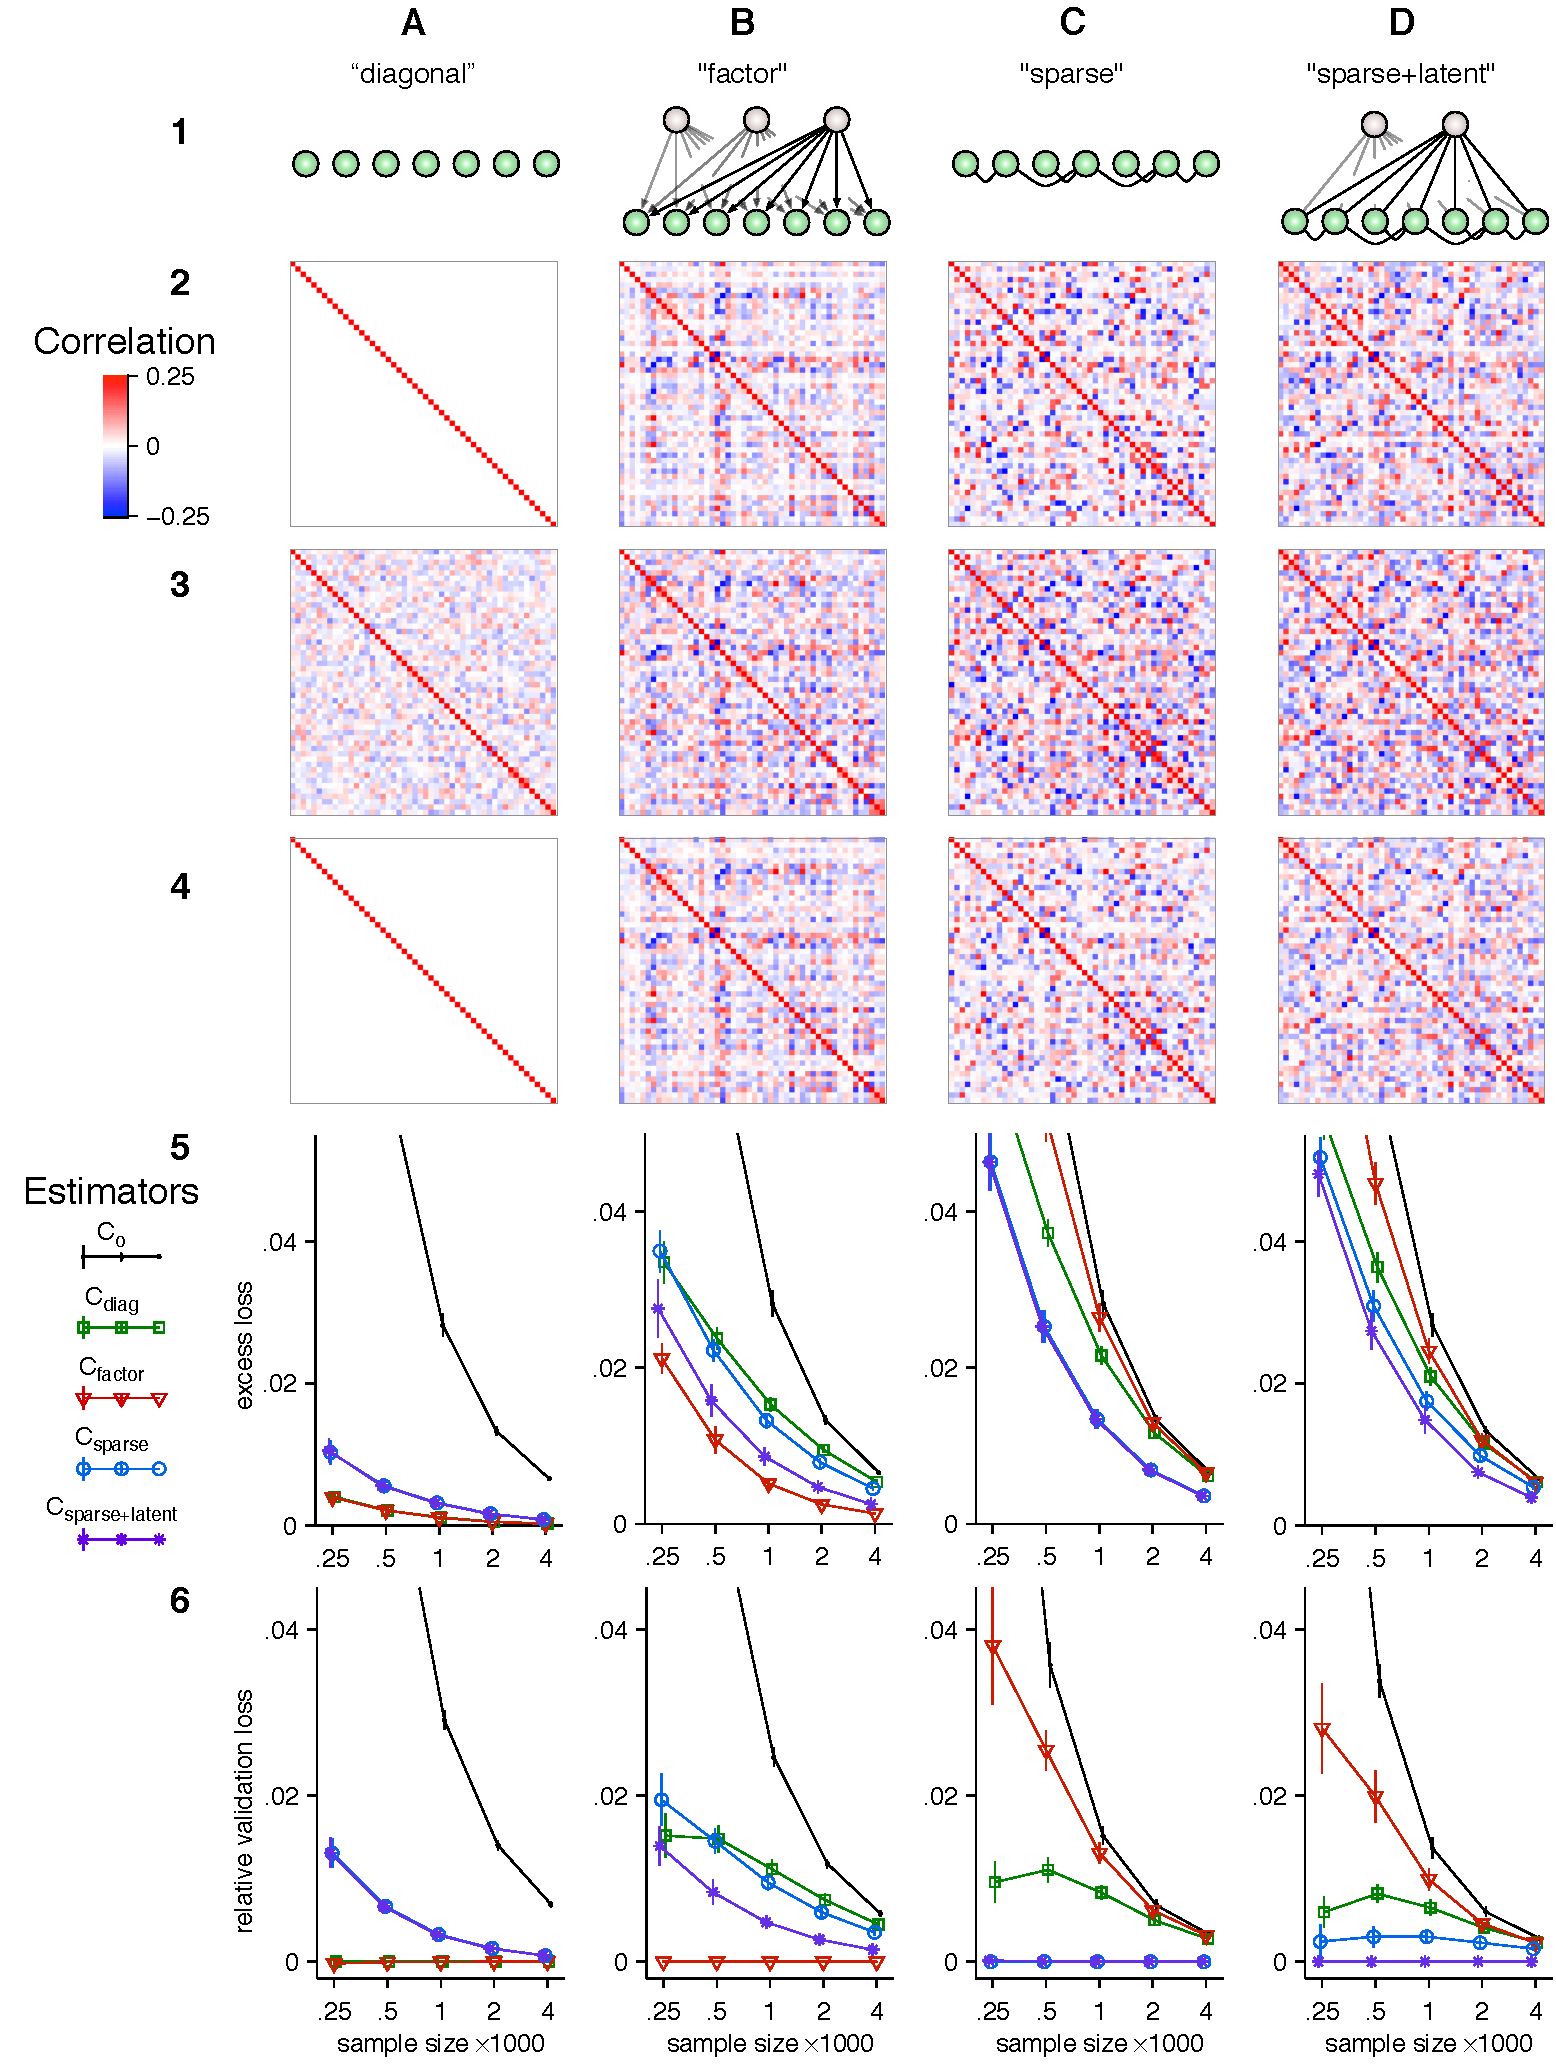
\includegraphics[width=\textwidth]{./figures/Simulation.pdf}
\end{fullpage}
\end{figure}
